
We explain the in-vehicle setup and implementation of EcoDrive.


\subsection{In-vehicle Setup}


\begin{figure}[t]
\begin{center}
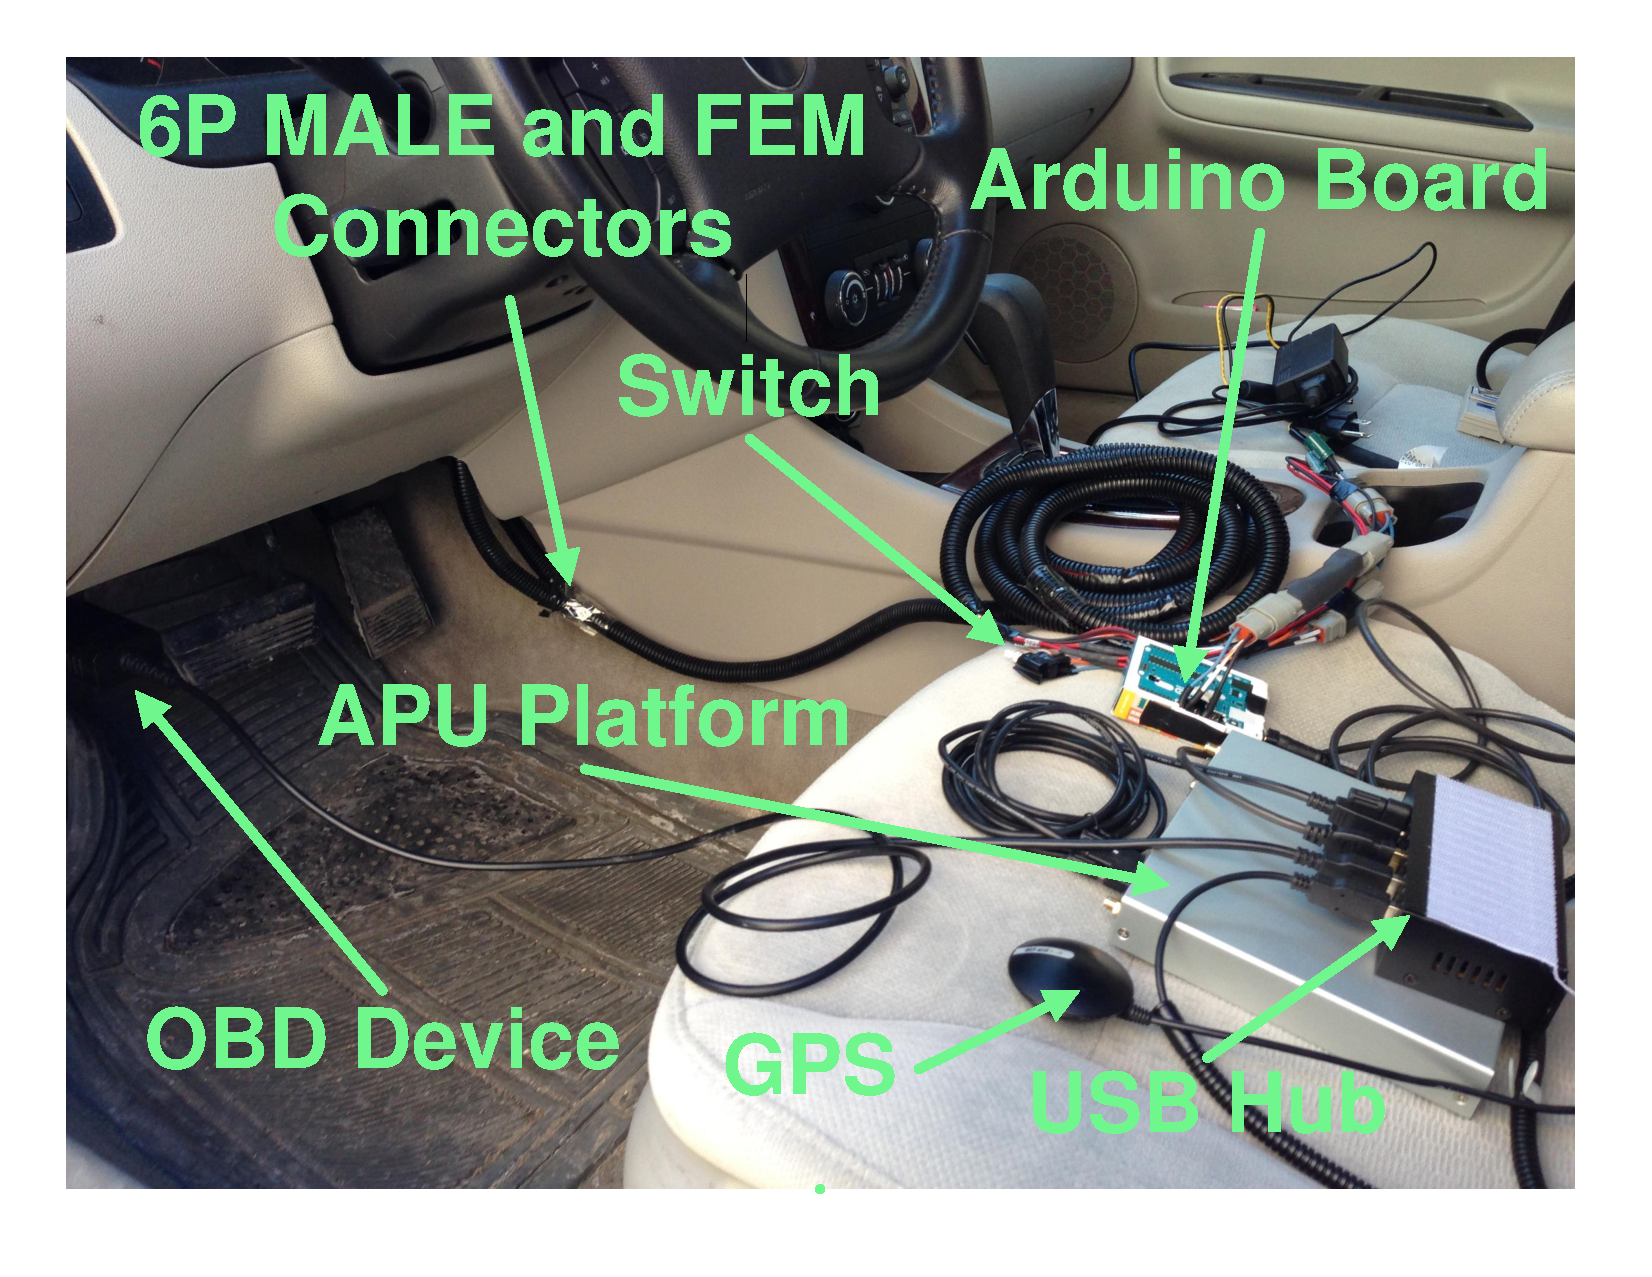
\includegraphics[width=3.0in,angle=0]{Figs/EcoDrive/setup_3.pdf}
\vspace{-0.3cm}
\caption{EcoDrive in-vehicle setup.}
\vspace{-0.6cm}
\label{setup}
\end{center}
\end{figure}


The in-vehicle setup of EcoDrive is shown in Fig. \ref{setup}. 
EcoDrive uses Arduino Uno microcontroller to emulate 
gas pedal by delivering signals to the ECU through a 6P FEM Connector. 
The microcontroller outputs a 16-bit resolution digital pulse-width modulation (PWM) 
signal which is smoothed out by an RC filter. 
A 6P MALE Connector is used to read signal outputs from 
the original gas pedal. 
A wiring harness and switch button are built that allows the user 
to switch the signal read by the ECU between the gas pedal and 
the microcontroller.  
Therefore, the setup supports two mode, human driving mode and
EcoDrive mode. 
In human driving mode, the gas pedal and air/fuel injection rate
is controlled by human driver.
In EcoDrive mode, the gas pedal is unusable and air/fuel injection rate
is controlled by the system. 
In EcoDrive mode, The APU platform \cite{apu} sends pedal positions to the microcontroller through 
serial communication and the microcontroller converts the pedal position values 
into analog voltages outputs. 
To do this, we construct a mapping between sensor analog 
voltage outputs and pedal positions. 
By using the mapping between gas pedal position
and air/fuel rate built from driving traces, 
we can send position values from laptop to the car
to control air/fuel injection rate.  

\vfill\eject

\subsection{Implementation}


We implement EcoDrive data sensing module and air/fuel
injection control module in C++. 
We operate EcoDrive on the Ubuntu 14.04 32bit distribution 
(with linux kernel version 3.13.0-34-generic), 
that runs on PC Engines APU platform \cite{apu}. 
APU platform is a mobile embedded platform that 
is equipped with 1GHz dual core CPU and 4G DDR3 DRAM. 
EcoDrive uses two threads to
query and read OBD messages, respectively. 
One thread sends OBD query message to the OBD port in every 250ms.
Higher frequency OBD query will cause CAN read error. 
Another thread listens on the OBD port for 
echo messages and sends voltage control commands to 
Arduino board. 
The Arduino board initiates a loop to listen on the USB 
serial and sets the voltage output of two pins 
based on received command. 
The two pins represent the voltage output pins
of gas pedal's two position sensors. 



\nop{
\subsection{OBD Data Collection}


\begin{figure}[!htbp]
\begin{center}
\vspace{-0.0cm}
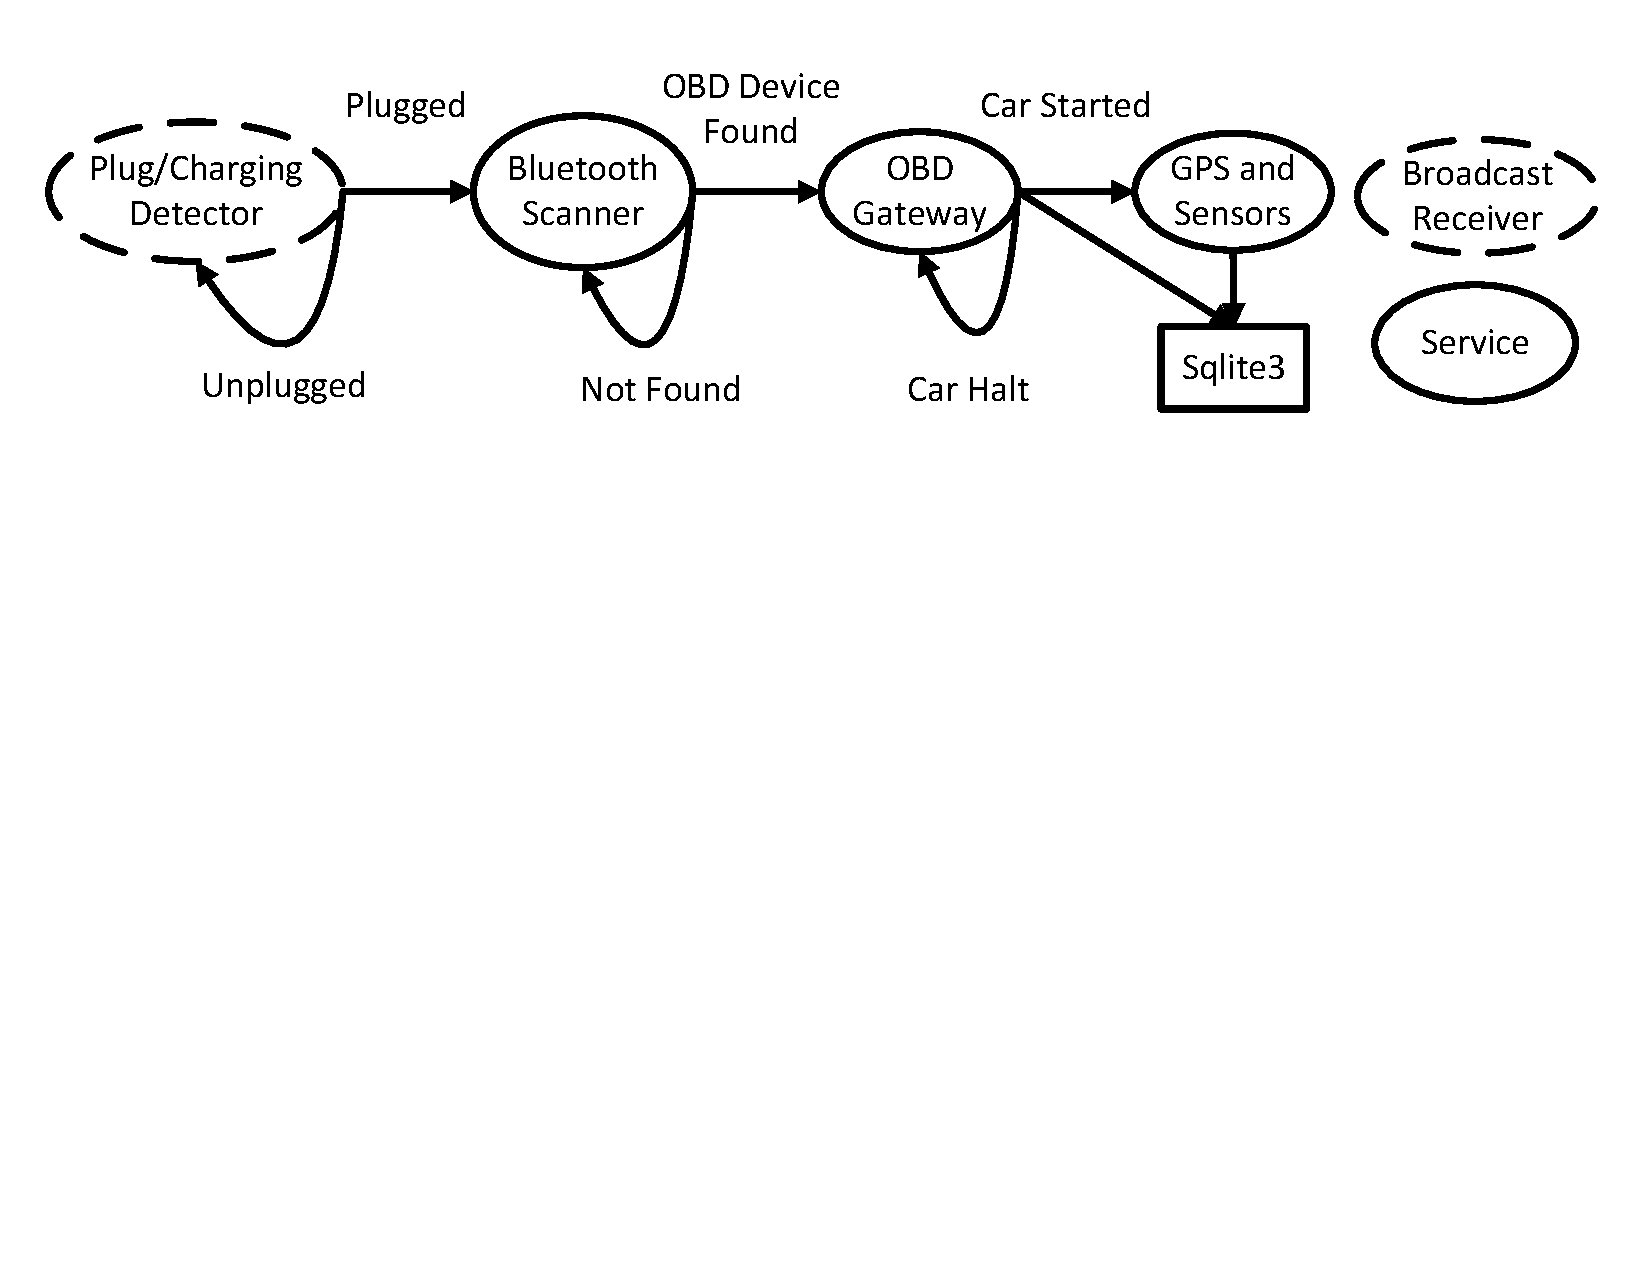
\includegraphics[width=3.0in,angle=0]{Figs/EcoDrive/datacollection.pdf}
\vspace{-5.0cm}
\caption{The control flow of Android application that is used for OBD data collection.}
\vspace{-0.4cm}
\label{data_collection}
\end{center}
\end{figure}

To collect driving data from different vehicles, 
we use Motorola Xoom with customized data collection
Android application.
Motorola Xoom is plugged with car charger adapter
and interacts with a standard bluetooth OBDII scan device. 
The control flow of the application is shown in Fig. \ref{data_collection}. 
In our setting, the tablet car charger adapter is always
plugged into the in-car charger outlet.  
Turning on the ignition will start charging the tablet, 
while some cars can still charge the tablet after car stalls, 
i.e., 2011 Chevrolet Impala, 2005 Buick LaCrosse etc. 
The plug/charging detector is a broadcast receiver to detect
the plug/charging status of the tablet. 
The broadcast receiver reads the charging status of 
the tablet periodically by using \emph{AlarmManager}. 
\emph{AlarmManager} can hold a CPU wake lock to guarantee that 
the tablet will not sleep and the application wakes up periodically.
The Bluetooth Scanner tries to connect to the OBD device. 
Once a bluetooth OBD device is found, 
the OBD Gateway sends OBD messages to test the engine
status of the car.
This is used to deal with the cars that the tablet is still charging
even after turning off the ignition. 
If the car engine is started, the application starts to write
the OBD messages and results into sqlite3 databases.  
GPS and other sensor data from the tablet are also collected. 
Each trip is recorded in a database file. 


}
